I förra kapitlet togs en differentialekvation fram som beskriver vårat system som en relation mellan insignalen och utsignalen. Utifrån denna differentialekvation kan nu olika systemegenskaper tas fram som gör det möjligt att analysera systemet. Systemet kommer regera olika beroende på systemparametrarna, exempelvis kommer linan svänga olika beroende på vikten av personen på linan.

Systemanalysen kommer titta närmare på följande funktioner: systemfunktionen, impulssvaret, stegsvaret, \textbf{(rampsvaret,)} frekvensfunktionen samt amplitud- och faskaraktäristiken.
Vissa av dessa funktioner tas fram med hjälp av olika transformer som existerar i frekvensdomänen vilket kommer diskuteras i nästa kapitel.

\textbf{(ny sida här för att få figuren på nästa sida att komma på rätt ställe, kanske går att fixa senare)}

\newpage
\subsection{Frekvensdomänen}
Tidigare i rapporten har vi sett på insignalen och utsignalen som funktioner av tid. Vi kommer nu behöva betrakta hur signalerna beter sig i frekvensdomänen där man istället kollar på vilka frekvenser som signal är uppbyggd av.

Till exempel kan signalen $x(t)=3sin(2t) + sin(4t)$ ses som summan av två amplituder i tidsdomänen. I frekvensdomänen skulle den dock vara uppdelad i dess frekvenskomponenter, i detta fall två stycken vid frekvenserna $2$ och $4$. Detta visas grafiskt i figuren nedan.

\begin{figure}[h] % h = here
    \centering
    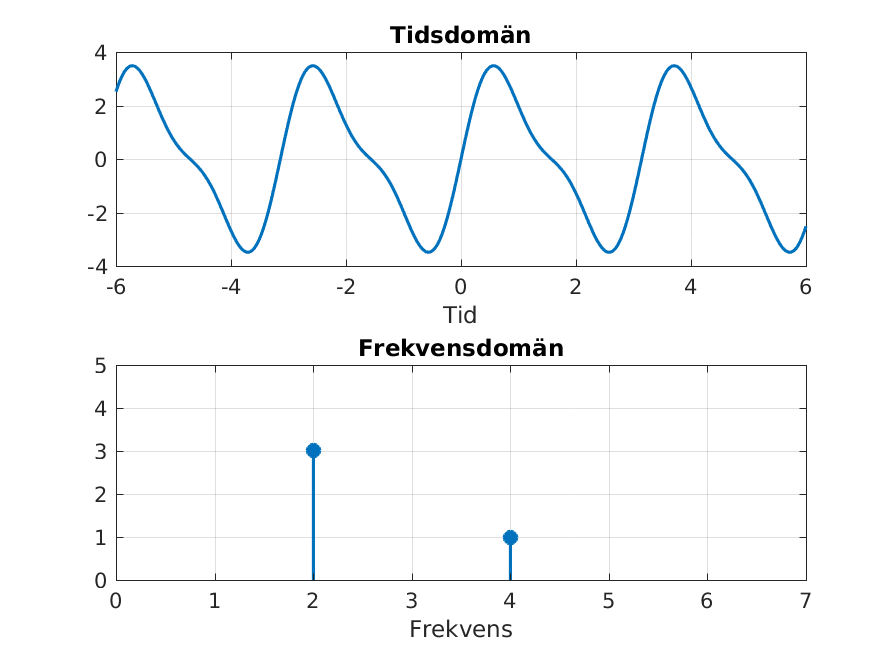
\includegraphics{bilder/tid_vs_frekvens_exempel}
    \caption{Tidsdoämen och frekvensdomänen av signalen $x(t)=3sin(2t)+sin(4t)$}
    \label{fig:tid_vs_frekvens_exempel}
\end{figure}

För systemanalysen kommer olika transformer som överför funktioner från tidsdomänen till frekvsensdomänen att användas, speciellt Laplacetransformen och Fouriertransformen.
Laplacetransformen är ett vanligt verktyg för att lösa differentialekvationer. För att ta sig tillbaka till tidsdomänen från frekvensdomänen kan inverstransformer appliceras.

\subsection{Systemfunktion}
Systemfunktionen beskriver ett förhållande mellan utsignalen och insignalen i frekvensdoämnen. Detta betyder att man kan räkna ut en utsignal om man vet insignalen i frekvensdoämnen och systemfunktionen. 
Detta går också att göra i tidsdomänen med faltning men det är oftast enklare att utföra beräkningen i frekvensdoämen.

För att beräkna systemfunktionen kommer hela differentialekvationen för systemet att Laplacetransformeras till frekvensdomänen. Det finns då två versioner av Laplacetransformen som kan användas: den enkelsidiga och den dubbelsidiga.
Eftersom .... (alltså att en utsignal inte beror på tidigare händerlser i system). Detta brukar kallas att systemet är kausault.
Den enkelsidiga Laplacetransformen för en funktion $x(t)$ definieras som:

$$X(s) = \mathcal{L}\big\{x(t)\big\} = \int\limits_{0-}^{\infty} x(t)e^{-st}\,dt$$

där s är en komplexvärd frekvens vanligtvis betecknad $s=\sigma+j\omega$.
Här används versaler för att beteckna funktioner i frekvensdomänen.
Denna transform behöver inte vara definierad för alla $s$ utan kan divergera i vissa fall. Därför är det viktigt att säga vart den transformerade funktionen är definierad. 

Eftersom dessa integralberäkningar kan bli både långa och krångliga kommer vi i denna rapport använda tabellerna i häftet \textit{Formler \& Tabeller}  \textbf{(insert referens)} för att beräkna Laplacetransformerna.
För att transformera differentialekvationen kommer följande samband för derivering i tidsdomänen att användas enligt tabell 18.7:
$$\mathcal{L}\bigg\{\frac{dy(t)}{dt}\bigg\} = sY(s)-y(0-)$$
Då vårat system är energifritt och alltså inte har några initialtilståd försvinner alla $y(0-)$-termer. Vår differentialekvation kan alltså Laplacetransformeras enligt:
$$ \mathcal{L}\bigg\{m\displaystyle\frac{d^2y(t)}{dt^2} + c\displaystyle\frac{dy(t)}{dt} + ky(t)\bigg\}= \mathcal{L}\bigg\{x(t)\bigg\} $$
\begin{center}$ \Longleftrightarrow \bigg/$ Tabell $18.7$, $18.8\,\bigg/$ \end{center}
$$ \Longleftrightarrow\, ms^2Y(s)+csY(s)+kY(s)=X(s)$$

Från ekvationen ovan kan nu systemfunktionen $H(s)$ bestämmas då den definieras som kvoten mellan utsignalen och insignalen i frekvensdomänen. Genom att bryta ut termen $Y(s)$ i vänsterledet och sedan dela med $X(s)$ och $s$-polynomet i båda led ges följande: 
$$H(s)=\frac{Y(s)}{X(s)}=\frac{1}{ms^2+cs+k}$$

\subsubsection{Pol-nollställediagram}
Utifrån systemfunktionen kan nu flera egenskaper om systemet tas fram. Oftast är det intressant att studera nollställerna för polynomerna i systemfunktionen. Nollställen i täljarpolynomet kallas systemfunktionens nollställen medan nollställen i nämnarpolynomet kallas systemfunktionens poler \textbf{(\textless- ful mening plz fix)}. Man kan direkt se att systemfunktionen inte har några nollställen då täljarpolynomet inte har några lösningar (\textbf{visst heter nollställen till ett polynom för lösningar?}). För att hitta polerna så måste rötterna till nämnarpolynomet hittas, detta kan göras med till exempel pq-formeln:
$$ms^2+cs+k=0$$
$$\Longleftrightarrow s=-\frac{c}{2m}\pm \sqrt{\bigg(\frac{c}{2m}\bigg)^2-\frac{k}{m}}$$

TODO: 3 fall, hänvisa till figur, nivåkonstant, konvergensområde, figurer, 3d figur.
Nämn ordet diskriminant, holy fuck vilket fancy ord:  \href{https://sv.wikipedia.org/wiki/Andragradsekvation#L.C3.B6sningsformeln}{Länk}


\subsection{Stabilitet}
antar vi att konstanerna $m, c, k >0$, vilket krävs för att systemet ska vara realiserbart, så är (börjar konvergensområdet på vänsta halvplanen och går till högra) 

\subsection{Impulssvar}
vad skulle detta vara fysikaliskt i vårat system?

TODO: kvadratkomplettera och förläng H(s) tills den den kan inverstransformeras enligt tabell

\subsection{Stegsvar}
(OBS: ska lösas med faltning)

Kommer behöva göra upprepad paritell integration (finns andra sett enligt Envar-1-boken men de verkar mer krångliga/svåra att härleda)

\subsection{Rampsvar}
Är detta relevant?
(förmodligen inte)

\subsection{Frekvensfunktion}


\subsection{Amplitud- och faskaraktäristik}


\subsection{Utsignal}
